\section{Simulation der 2D-DFT}
Zur Simulation der Signalverläufe von Hardwarekomponenten dient in der Cadence-Umgebung das Programm NC\,Sim.
Das Programm beherrscht lediglich bei einzelnen Vektoren die Umrechnung zu vorzeichenbehafteten Zahlen im Dezimalsystem.
Bei der Bündelung von Vektoren können nur positive Dezimalzahlen dargestellt werden. Dies hat zur Folge, dass Vektoren, die eine negative Zahl repräsentieren, mittels $2^{n+1}+m$, $n=$ Bitbreite des Vektors und $m=$ angezeigte Zahl, bei Bedarf händisch umgerechnet werden müssten. 
Die Darstellung von Festkoomazahlen ist in keinem Fall möglich.

 Anhand der Simulation kann die Anzahl der im Voraus ermittelten, zur Berechnung der 2D-DFT benötigten Takte, verifiziert werden, was nachfolgend geschen soll.
 
 Nachdem \texttt{nReset} auf '1' gesetzt wird, werden die Eingangswerte
 eingelesen. Wenn dieser Vorgang abgeschlossen ist, geht \texttt{loaded} auf '1'. Mit der nächsten steigenden Taktflanke, in Bild \ref{pic:Simulationsdauer} bei 
 \SI{340}{ns}, beginnt die Berechnung
 der \gls{2d-dft}. Beendet ist sie, nachdem die Matrizenmultiplikation auf die Eingangswerte und anschließend auf die \gls{1d-dft}-Werte angewandt wurde. Also nach $2 \cdot 64$
 einzelnen Berechnungen. Wenn dies erfolgt ist, wird \texttt{result\_ready} auf '1' gesetzt. Dies geschieht bei \SI{20\,820}{ns}. Bei einer Taktfrequenz von $(\SI{40}{ns})^{-1}$
 (siehe \ref{src:dft8_optimiert_top}) ergeben sich so 512 Takte. Dies bestätigt auch der Edge Count, ebenfalls auf dem Bild zu sehen, welcher die Flanken des \texttt{clk}-Signals 
 zählt. In der Simulation ist zu erkennen, dass die Berechnung der Elemente 
 unterschiedlich viele Takte beansprucht. Hieran lässt sich ebenfalls sehen, dass die 1. (ungerade) Zeile weniger Takte gegenüber der 2. (geraden) Zeile benötigt. 
 
 %Auch in der Abbildung \ref{pic:Simulationsdauer} zu sehen ist, dass \texttt{element\_out} für 0 bis 7 weniger Takte einnimmt, als in den darauf folgenden 8. Dieses Muster
 %wiederholt sich und hat, wie in Abschnitt \ref{sec:berechnung_anzahl_takte} erläutert, damit zu tun, dass für die geraden
 
 \begin{figure}[htbp]
  \centering
  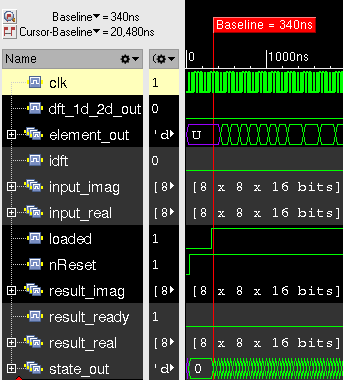
\includegraphics[width=0.58\textwidth]{img/Simulationsdauer_Anfang.png}
  \hfill
  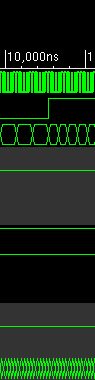
\includegraphics[width=0.161\textwidth]{img/Simulationsdauer_Mitte.png}
  \hfill
  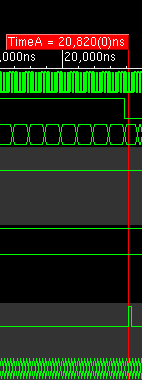
\includegraphics[width=0.241\textwidth]{img/Simulationsdauer_Ende.png}
  \caption{Ausschnitt des Simulationstools \texttt{NC\,Sim} von der Berechnung und Verifikation der 2D-DFT.}
  \label{pic:Simulationsdauer}
 \end{figure}

 \begin{figure}[htbp]
  \centering
  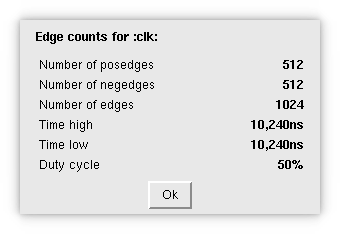
\includegraphics[width=0.6\textwidth]{img/Simulation_edge_count_clk.png}
  \caption{Edge Count des Taktsignals für die vollständige Simulation der 2D-DFT.}
 \end{figure}

 \section{Zeitabschätzung als Winkelsesnor im Antriebsmotor eines Elektroautos}
 Anhand der nun bekannten Größe von 512 Takten kann ermittelt werden, ob die Implemenatation vom zeitlichen Aspekt her akzeptabel ist.
 Die maximale Drehzahl eines Elektromotors wird laut Datenblatt der Firma ABM Greiffenberger mit 8000\,U/min angegeben~\autocite[5]{greiffenberger},
 als maximale Taktfrequenz des Sensors ist 100\,MHz vorgegeben.
 
%  \begin{equation*}
%    RPM = 8000\, \textrm{min}^{-1}
% \end{equation*}

% \begin{equation}
%  \begin{split}
%   \frac{RPM}{60} = 1333,\bar{3}\,\texttt{sec}^{-1}  \\
%  \end{split}
% \end{equation}

%  \begin{equation}
%   \curvearrowright 1\, \textrm{Umdrehung} = 7,5\cdot 10^{-3}\,\textrm{sec}
%  \end{equation}
 
 \begin{equation}
 \begin{split}
    RPM &= 8000\, \textrm{min}^{-1}\\[10pt]
    \frac{RPM}{60} &= 1333,\bar{3}\,\texttt{sec}^{-1}  \\[10pt]
    \curvearrowright 1\, \textrm{Umdrehung} &= 7,5\cdot 10^{-3}\,\textrm{sec}\\[10pt]
    1^\circ &\widehat{=} \frac{7,5\cdot 10^{-3}\,\textrm{sec}}{360}\\[10pt]
    1^\circ & \widehat{=} 20,83\cdot10^{-6}\,\sec \\[10pt]
    100\cdot10^6\,Hz &= 10\cdot10^{-9}\,\sec \\[10pt]
    \frac{20,83\cdot10^{-6}}{10\cdot10^{-9}} &= 2083
    \end{split}
 \end{equation}


 Um eine Aussage über die restliche zur Verfügung stehenden Zeit bzw. Takte machen zu können, wird gezeigt, dass pro Winkel 
 etwa 2080 Takte für Berechnungen zu Verfügung stehen.
 Da 512 etwa 25$\%$ von 2083 sind, resultiert hieraus, dass noch etwa 75$\%$ der Takte nutzbar sind. Wenn auch die IDFT durchgeführt werden muss, bleibt die Hälfte
 der verfügbaren Takte für Interpolation, Filterung, Berechnung so wie Ausgbae bzw. Übertragung des Winkels.

 
\section{Test der Matrixmultiplikation}


\subsubsection{1D-DFT mit Integer-Werten}
 
\subsubsection{2D-DFT mit Integer-Werten}

\subsubsection{2D-DFT mit Werten SQ-Format}

Unter anderem weil NC\,Sim bzw. dessen Unterprogramm SimVision zur Anzeige von Signalverläufen (Waveform) nur Integer darstellen kann und bei als Vektor gebündelten Signalen 
diese nicht einmal als vorzeichenbehaftet (signed), wurde der Einfachheit halber zunächst die Berechnung als Ganzzahl-Multiplikation mit dem Faktor 3 betrachtet. 
Da es bei diesem Faktor und den gewählten Eingangswerten nicht zu einem 
Überlauf kommen kann, war es zu diesem Zeitpunkt noch nicht nötig, sich Gedanken über die Breite des Ergebnisvektors bzw. den Ausschnitt daraus für die weitere
Berechnung zu machen. Deshalb konnte an dieser Stelle noch auf den Bitshift zur Halbierung der Werte verzichtet werden.

Erst als der Faktor $\frac{\sqrt{2}}{2}$ übernommen wurde, wurden die Ergebnisse breiter als der Vektor für die weitere Berechnung an Bits zur Verfügung stellt.

${\frac{\sqrt{2}}{2}}_{10}$ = $0001011010100_2$ in S2Q10, als Integer betrachtet jedoch $724_{10}$.

Daraus folgt, dass ein Teil der Bits abgeschnitten werden müssen. Da die Dualzahlen jetzt im S1Q10-Format betrachtet werden, es sich also um Kommazahlen handelt,
müssen die hinteren Bits abgeschnitten werden. Zudem können vorne Bits ohne Informationsverlust gestrichen werden, da durch die Multiplikation ein weiteres 
Negations-Bit dazugekommen ist und auf Grund des gegebenen Faktors der Wertebereich vorne nie ganz ausgenutzt wird. (Verifizieren / Belegen!)

 